\documentclass[10pt]{article}
\usepackage[spanish,mexico]{babel}
\usepackage[T1]{fontenc}
\usepackage[utf8]{inputenc}
\usepackage{lmodern}
\usepackage{microtype}
\usepackage[a4paper,margin=2.15cm,headheight=14pt,headsep=18pt,footskip=27pt]{geometry}
\usepackage{amsmath,amssymb}
\usepackage{graphicx}
\usepackage{booktabs,tabularx,array}
\usepackage{xcolor}
\usepackage{titlesec}
\usepackage{fancyhdr}
\usepackage{caption}
\usepackage{xurl}
\usepackage{hyperref}
\hypersetup{colorlinks=true,linkcolor=blue!45!black,citecolor=blue!45!black,urlcolor=blue!55!black}
\setlength{\parskip}{4pt}
\setlength{\parindent}{0pt}
\setlength{\emergencystretch}{2em}
\setcounter{secnumdepth}{2}
\setcounter{tocdepth}{1}
\titleformat{\section}{\large\bfseries\color{blue!45!black}}{\thesection}{.6em}{}[\color{blue!20!black}\titlerule]
\titleformat{\subsection}{\normalsize\bfseries\color{blue!40!black}}{\thesubsection}{.6em}{}
\titlespacing*{\section}{0pt}{1.45em}{.55em}
\titlespacing*{\subsection}{0pt}{1.05em}{.35em}
\captionsetup{font=small,labelfont=bf,justification=centering,singlelinecheck=false}
\pagestyle{fancy}
\fancyhf{}
\fancyhead[L]{\small Skyntists · AstroHack SATEM 2026}
\fancyhead[R]{\small Memoria técnica}
\fancyfoot[C]{\thepage}
\renewcommand{\headrulewidth}{.4pt}
\renewcommand{\footrulewidth}{0pt}

\title{\vspace{-1.3em}\textbf{Análisis técnico de líneas moleculares en IRAS 16293--2422 B}\\[.35em]
\large Memoria ampliada del proyecto AstroHack SATEM 2026}
\author{Equipo Skyntists\\Angel Gabriel Jiménez Isidro · Carlos Manuel Martínez Hernández\\Luis Gustavo Cons · Paola Díaz Arellano\\\small Yarek Alejandro Olivares Meneses}
\date{Versión técnica ampliada · Octubre de 2026}

\begin{document}
\maketitle
\begin{abstract}
Esta memoria documenta el flujo de análisis aplicado a dos ventanas espectrales ALMA, W1 y W2, de la fuente joven IRAS 16293--2422 B. El objetivo es evaluar si rasgos observados son compatibles con transiciones de moléculas de interés prebiótico, dejando trazabilidad entre archivos calibrados, frecuencias de catálogo, perfiles ajustados y decisiones de evidencia. Se verifica la extracción B\_offset contra los cubos FITS cuando están disponibles, se estima ruido local con MAD de primeras diferencias, se buscan máximos por prominencia y se comparan con frecuencias de reposo mediante la convención de velocidad radio. Se obtienen 107 asociaciones catálogo--pico agrupadas en 64 rasgos coincidentes; seis perfiles seleccionados son compatibles de forma tentativa con CH$_3$CN o CH$_3$CHO. Una coincidencia de glicina-I en una región congestionada se conserva como resultado insuficiente. No se afirma detección confirmada, abundancia, temperatura de excitación ni evidencia de vida. El catálogo local es parcial y el SNR es local y aproximado, por lo que se explicitan los límites de inferencia y los pasos requeridos para robustecer el resultado.
\end{abstract}

\textbf{Nota de alcance.} Este documento complementa el informe breve requerido por la convocatoria (2--3 páginas más referencias); no lo sustituye. Su propósito es apoyar la revisión técnica, la reproducibilidad y la defensa oral.

\tableofcontents
\newpage

\section{El reto y la pregunta de investigación}
El AstroHack SATEM 2026 propone examinar datos reales de ALMA para encontrar moléculas de interés prebiótico, justificar las asignaciones y discutir su posible relación con la química anterior al surgimiento de la vida. La tarea central no es contar coincidencias aisladas: consiste en mostrar cómo una frecuencia medida puede compararse con datos de laboratorio y cuánto peso merece la interpretación después de considerar movimiento del gas, ruido, perfiles superpuestos y especies alternativas.

La pregunta de este proyecto es: \emph{¿contienen los espectros entregados hacia IRAS 16293--2422 B rasgos compatibles con varias transiciones de CH$_3$CN y CH$_3$CHO, y qué grado de confianza permite la evidencia disponible?} Se trata de una prueba de compatibilidad con un catálogo educativo seleccionado, no de una búsqueda exhaustiva de todas las especies ni de una medición de composición química absoluta.

\subsection{Requisitos y criterios del reto}
La guía del participante pide un informe de 2--3 páginas más referencias, con pregunta, método, espectros comentados, interpretación astrobiológica, tabla breve de candidatas, líneas que respaldan cada propuesta, catálogo y confianza declarada. También requiere declarar el uso de IA tanto en el informe como en la presentación y entregar materiales suficientes para repetir el análisis, además de reconocer las aportaciones individuales.

La evaluación indicada en la guía distribuye 100 puntos entre identificación molecular (25), interpretación astrobiológica (20), creatividad y herramientas (25), presentación y defensa (20), y claridad y autoría (10). Este proyecto responde a esos criterios con comparaciones Doppler trazables, una herramienta de análisis y comunicación, una interpretación prudente y un registro explícito de incertidumbres y uso de IA. Las contribuciones individuales siguen pendientes de completar por cada integrante; por ello no se asignan responsabilidades nominales en esta memoria.

\section{Contexto astrofísico y procedencia de los datos}
IRAS 16293--2422 es un sistema de formación estelar en la nube L1689N de Ofiuco. La fuente B se destaca por su espectro rico en líneas y por perfiles relativamente estrechos frente a la fuente A, rasgos que ayudan a separar transiciones cercanas, aunque no eliminan los blends. La investigación PILS documentó la complejidad molecular de este sistema con ALMA [1]. La abundancia de líneas hace que el entorno sea valioso para la astroquímica y también aumenta la posibilidad de confusión entre especies.

El paquete educativo deriva del proyecto ALMA ADS/JAO.ALMA\#2013.1.00278.S y contiene productos procesados ARI-L. De acuerdo con la guía, los espectros se entregan calibrados y extraídos; el trabajo del reto se centra en interpretarlos, no en volver a calibrar las observaciones. Las tablas están en Jy/beam y en el marco LSRK. Los CSV contienen tres extracciones: B\_offset, B\_pico y A. El análisis de candidatas de esta memoria usa B\_offset, posición recomendada por la guía y apartada del máximo de continuo. Las ventanas W1/W2 tienen haces diferentes; sus intensidades no se interpretan como abundancias comparables.

\begin{table}[!htbp]
\centering\small
\caption{Cobertura y muestreo de las extracciones espectrales utilizadas.}
\begin{tabular}{@{}lrrrrl@{}}
\toprule
Ventana & Canales & Frecuencia mínima (MHz) & Frecuencia máxima (MHz) & Paso (MHz) & Unidad de intensidad\\
\midrule
W1 & 1\,918 & 348\,834.4483 & 349\,302.4456 & 0.2441 & Jy/beam\\
W2 & 1\,918 & 349\,303.1814 & 349\,771.1787 & 0.2441 & Jy/beam\\
\bottomrule
\end{tabular}
\end{table}

Los nombres de archivo principales son \texttt{espectros/W1\_espectros.csv}, \texttt{espectros/W2\_espectros.csv}, \texttt{catalogos/catalogo\_local\_prebioticas.csv} y \texttt{Entregables/Campos\_de\_evidencia.csv}. Los productos FITS conservan el cubo y sus metadatos; los CSV son espectros extraídos de una posición y no contienen por sí solos la información espacial completa.

\subsection{Verificación de la extracción}
Cuando los FITS están presentes, el notebook inspecciona el cubo y comprueba la dimensionalidad, el número de canales, la unidad \texttt{BUNIT=Jy/beam} y el marco \texttt{SPECSYS=LSRK}. Después compara el espectro del píxel $(x,y)=(54,46)$ con la columna B\_offset del CSV mediante \texttt{numpy.allclose} con tolerancias relativas y absolutas explícitas. Esta verificación puede detectar errores de lectura, correspondencia del píxel o unidades; no recalibra los datos ni valida una identificación molecular. Si falta un cubo, el flujo registra que se usa la extracción CSV suministrada.

\begin{figure}[!htbp]
\centering
\IfFileExists{figuras/espectros_completos.png}{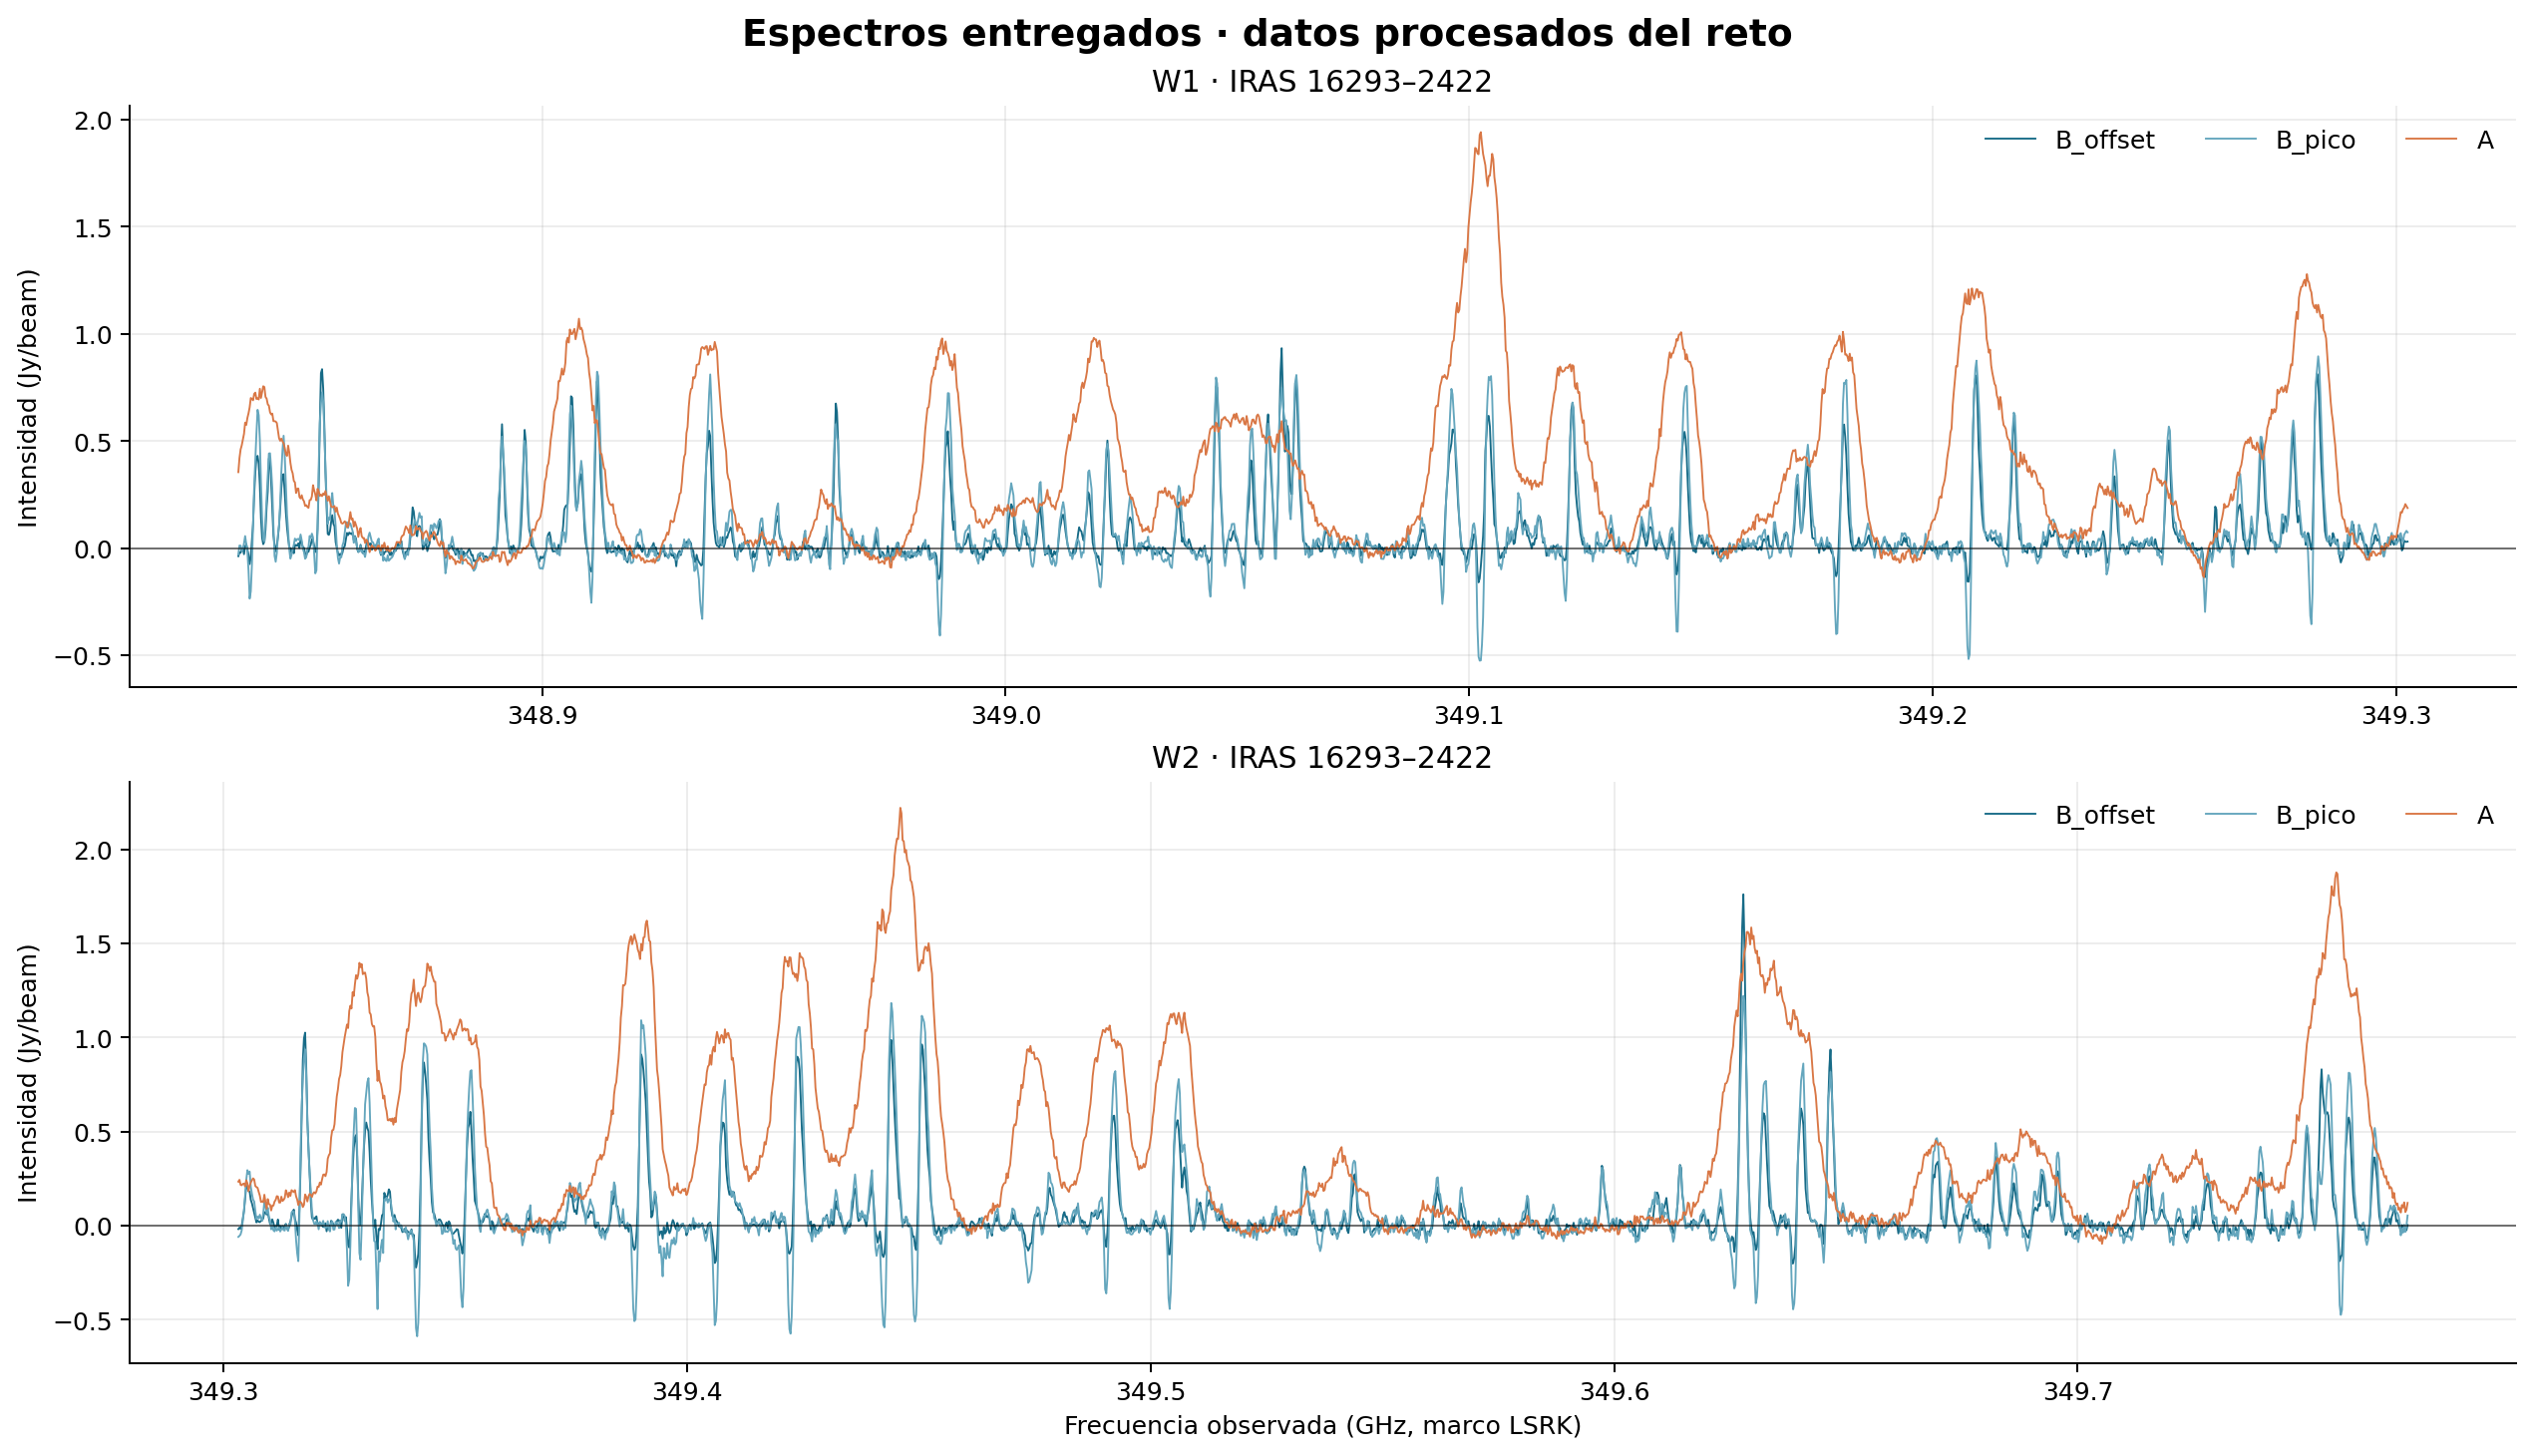
\includegraphics[width=.94\linewidth]{figuras/espectros_completos.png}}{\fbox{Ejecutar el notebook para generar \texttt{figuras/espectros\_completos.png}}}
\caption{Espectros completos entregados para las extracciones disponibles. El eje de frecuencia ya está expresado en LSRK; la comparación con frecuencias de reposo requiere aplicar una única corrección por la velocidad de la fuente. Las ventanas tienen resoluciones angulares distintas.}
\end{figure}

\section{Método de análisis reproducible}
El notebook \texttt{herramientas/Inicio\_AstroHack.ipynb} organiza el procedimiento en etapas que permiten inspeccionar entradas, parámetros y productos derivados. A continuación se definen las transformaciones esenciales y sus supuestos.

\subsection{Control de estructura y unidades}
Se validan las columnas requeridas en cada espectro, la finitud y monotonía creciente del eje de frecuencia, y el número de muestras. El eje de los CSV está en GHz; para buscar contra catálogos se transforma a MHz mediante $1\,\mathrm{GHz}=10^3\,\mathrm{MHz}$. La intensidad se conserva en Jy/beam, sin reescalar una ventana respecto de otra.

\subsection{Estimación robusta del ruido}
Para una serie de intensidades $y_i$, se forman diferencias adyacentes $d_i=y_{i+1}-y_i$. El estimador empleado es
\begin{equation}
\widehat{\sigma}=\frac{1.4826}{\sqrt{2}}\,\operatorname{MAD}(d_i),\qquad
\operatorname{MAD}(d_i)=\operatorname{mediana}\left(\left|d_i-\operatorname{mediana}(d)\right|\right).
\end{equation}
El factor 1.4826 hace consistente la MAD con la desviación estándar para ruido gaussiano; dividir entre $\sqrt{2}$ compensa la varianza de una diferencia de dos canales independientes de varianza común. El método es resistente a valores atípicos y parte de la señal de línea se atenúa al diferenciar. No obstante, correlación entre canales, emisión extendida, baseline curvado o ruido no estacionario rompen esos supuestos. Así, $\widehat{\sigma}$ es una escala local aproximada y no incluye errores de calibración ni covarianza espectral.

\subsection{Detección de máximos}
En cada ventana se buscan máximos locales con \texttt{scipy.signal.find\_peaks}. El umbral de prominencia es el mayor entre $5\widehat{\sigma}$ y 0.03 Jy/beam; se exige separación mínima de tres canales. La prominencia mide cuánto sobresale el máximo de su entorno, no es idéntica a la altura del pico ni constituye significancia global corregida por haber buscado en muchos canales. La selección automática produce 64 máximos en W1 y 56 en W2 bajo esta configuración.

\subsection{Comparación con el catálogo y corrección Doppler}
La guía recomienda para B una velocidad inicial radio de $v_{\rm sys}=2.7$ km/s; el notebook explora un margen de $\pm1$ km/s. Para velocidades pequeñas frente a la velocidad de la luz, la frecuencia predicha en el marco LSRK se calcula como
\begin{equation}
\nu_{\rm pred,LSRK}=\nu_{\rm rest}\left(1-\frac{v_{\rm sys}}{c}\right),\qquad c=299\,792.458\;\mathrm{km\,s^{-1}}.
\end{equation}
La corrección se aplica una sola vez: el espectro ya está indicado en LSRK, pero el catálogo tabula frecuencia de reposo. Para cada transición dentro de la cobertura se elige el máximo candidato más cercano. La diferencia es
\begin{equation}
\Delta\nu=\nu_{\rm pico,LSRK}-\nu_{\rm pred,LSRK}.
\end{equation}
La tolerancia de asociación combina el margen de velocidad, la incertidumbre de catálogo cuando es positiva y medio canal:
\begin{equation}
\tau_0=\sqrt{\left(\nu_{\rm pred,LSRK}\frac{\Delta v}{c}\right)^2+
\sigma_{\rm cat}^{2}+\left(\frac{\delta\nu_{\rm canal}}{2}\right)^2}.
\end{equation}
Si la incertidumbre de catálogo está ausente o es cero, se trata como no informada, no como exacta. La tolerancia operacional se restringe al intervalo de un canal a 1.5 MHz para que una incertidumbre muy grande no se convierta en aceptación automática. Se conserva una asociación si $|\Delta\nu|\leq\tau$ y la prominencia supera $5\widehat{\sigma}$. Esta regla es una búsqueda de candidatas, no una prueba de identidad.

\subsection{Agrupación de asociaciones y ajuste de perfiles}
Varias transiciones catalogadas pueden señalar el mismo máximo. Se agrupan por rasgo/canal para no contar cada coincidencia como evidencia espectral independiente. En total, la tabla de asociaciones registra 107 pares catálogo--pico agrupados en 64 rasgos únicos (34 en W1 y 30 en W2). Estos conteos no deben confundirse con los 120 máximos locales detectados antes de consultar el catálogo.

Se seleccionaron seis perfiles visibles en B\_offset, tres para cada hipótesis molecular. Alrededor de cada frecuencia predicha se toma una región local de $\pm1.5$ MHz y se ajusta una gaussiana con baseline constante:
\begin{equation}
I(\nu)=b+A\exp\left[-\frac{(\nu-\mu)^2}{2s^2}\right],\qquad A\geq0.
\end{equation}
El ajuste no incluye una segunda componente para blends. La desviación espectral $s$ se restringe a 0.08--3 MHz y el centro $\mu$ a la ventana local. El ancho a mitad de altura se convierte a velocidad radio y el área gaussiana integrada se calcula como
\begin{align}
\mathrm{FWHM}_{\rm km/s}&=\frac{c}{\nu_{\rm rest}}\,2\sqrt{2\ln2}\,s,\\
W&=A s\sqrt{2\pi}\,\frac{c}{\nu_{\rm rest}}.
\end{align}
Con esta parametrización, la SNR reportada para perfiles ajustados es $A/\widehat{\sigma}$. No es la misma variable que la SNR de prominencia usada durante la búsqueda de máximos. El CSV etiqueta la incertidumbre de área como aproximada y advierte que no incorpora correlación entre canales, calibración ni incertidumbre de modelo.

\section{Resultados cuantitativos}
La tabla presenta las seis mediciones seleccionadas. $\Delta\nu$ se calcula respecto de la frecuencia de reposo corregida a LSRK con 2.7 km/s. Un valor positivo indica que el centro ajustado queda a frecuencia mayor que esa predicción. Esta comparación es derivada de las frecuencias tabuladas y ajustadas, no una segunda medición independiente.

\begin{table}[!ht]
\centering\footnotesize
\caption{Perfiles ajustados en B\_offset y evidencia asociada. La SNR es contraste local aproximado.}
\begin{tabularx}{\linewidth}{@{}l r r r r r r X@{}}
\toprule
Especie & Ventana & $\nu_{\rm rest}$ (MHz) & $\nu_{\rm fit}$ (MHz) & $\Delta\nu$ (MHz) & $v_{\rm radio}$ (km/s) & FWHM (km/s) & SNR\\
\midrule
CH$_3$CN & W1 & 349024.9709 & 349021.9375 & +0.1100 & 2.606 & 1.023 & 25.8\\
CH$_3$CN & W1 & 349125.2874 & 349122.2568 & +0.1137 & 2.602 & 1.166 & 34.2\\
CH$_3$CN & W2 & 349346.3430 & 349343.4907 & +0.2940 & 2.448 & 1.919 & 58.1\\
CH$_3$CHO & W1 & 348855.5714 & 348852.5305 & +0.1009 & 2.613 & 1.136 & 44.4\\
CH$_3$CHO & W2 & 349320.3515 & 349317.4912 & +0.2858 & 2.455 & 1.272 & 48.3\\
CH$_3$CHO & W2 & 349755.7020 & 349753.0048 & +0.4528 & 2.312 & 2.323 & 48.2\\
\bottomrule
\end{tabularx}
\end{table}

Las seis entradas se asocian con CDMS 41505 para CH$_3$CN y JPL 044003 para CH$_3$CHO. Sus velocidades inferidas se sitúan entre 2.31 y 2.61 km/s, próximas al valor inicial de 2.7 km/s, aunque no idénticas. La diferencia entre perfiles puede reflejar incertidumbre del centro, mezcla, baseline, selección local o diferencias físicas; no se estima aquí un parámetro sistémico global. La amplitud y SNR elevadas ayudan a localizar estructura en el espectro, pero no separan por sí mismas contribuciones de especies diferentes.

\begin{figure}[!ht]
\centering
\IfFileExists{figuras/perfiles_candidatos.png}{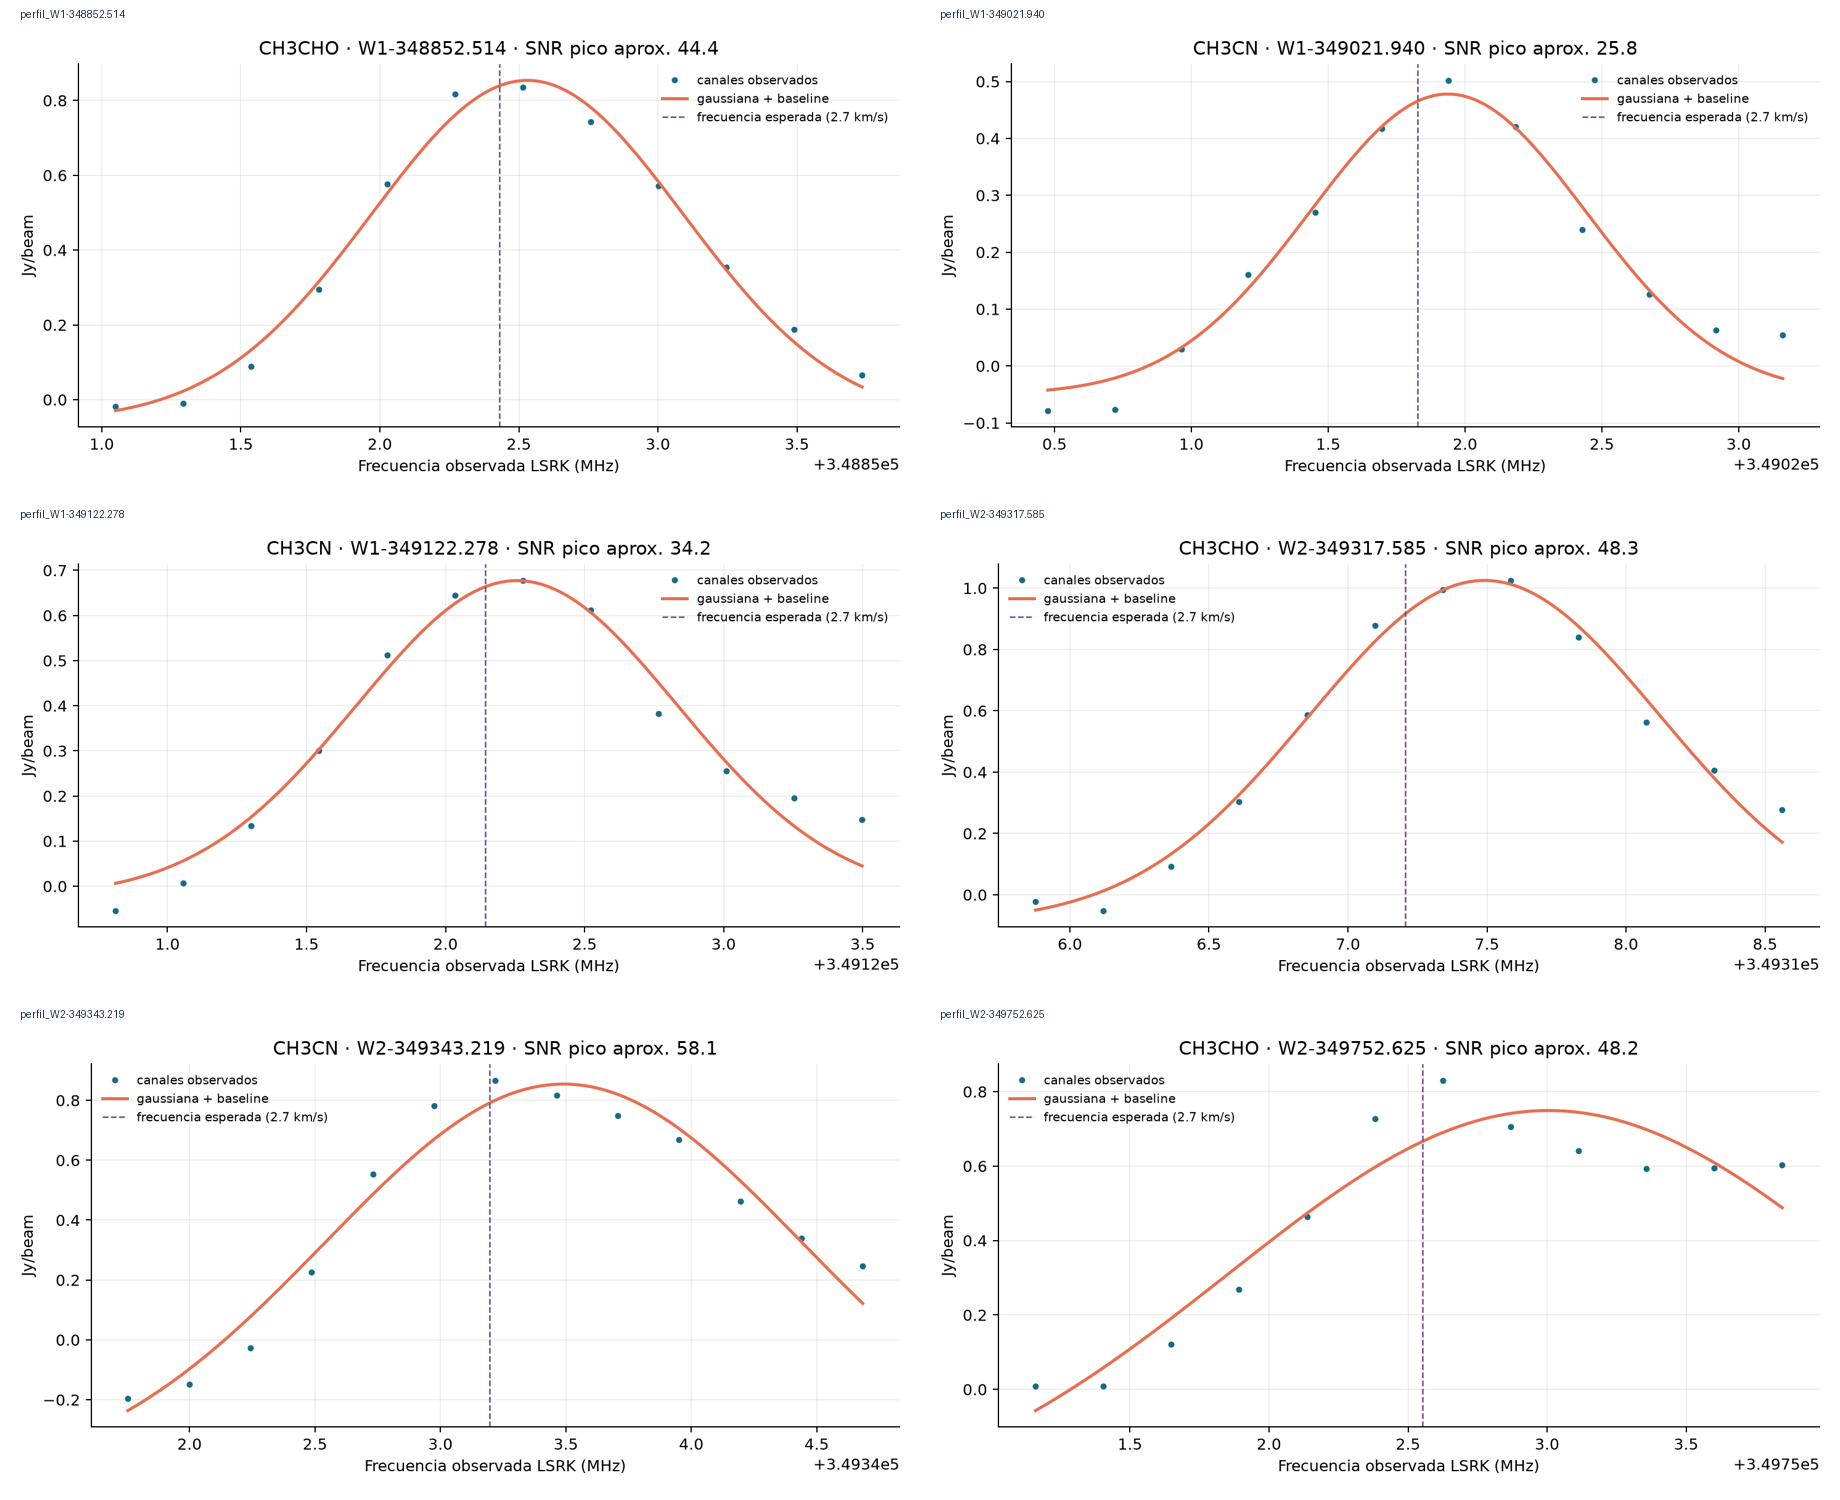
\includegraphics[width=.92\linewidth]{figuras/perfiles_candidatos.png}}{\fbox{Ejecutar el notebook para generar \texttt{figuras/perfiles\_candidatos.png}}}
\caption{Seis perfiles con el ajuste gaussiano descriptivo y la predicción cinemática del catálogo. El modelo de una componente no resuelve mezclas.}
\end{figure}

\subsection{Resultado alternativo: glicina-I}
Se conserva una coincidencia de catálogo CDMS 075511 con una estructura alrededor de 348\,963.349 MHz. La frecuencia de reposo es 348\,965.1769 MHz y la incertidumbre de catálogo comunicada es 0.766 MHz; la estructura cae en una zona congestionada y existen transiciones alternativas próximas. No se ajusta ni se atribuye el rasgo de forma exclusiva a glicina-I. El veredicto registrado es \emph{insuficiente}: una coincidencia aislada no demuestra varias transiciones independientes de la especie.

\section{Qué significa la evidencia molecular}
Una asignación robusta requiere que varias transiciones de una misma especie coincidan con frecuencias observadas después de una corrección cinemática consistente, que los perfiles puedan distinguirse de blends y que intensidades relativas sean plausibles bajo un modelo de excitación. La tabla de este proyecto usa seis rasgos seleccionados como hipótesis de trabajo; no se ha hecho una búsqueda ciega corregida por comparaciones múltiples ni una evaluación completa de especies contaminantes. El umbral de 5 en una estadística local no equivale a una tasa global de falso positivo conocida.

En consecuencia, la conclusión calibrada es que los seis perfiles son \emph{compatibles tentativamente} con transiciones de CH$_3$CN y CH$_3$CHO dentro de la selección y supuestos actuales. No se declara que la molécula esté confirmada en la fuente por este análisis, ni que la tabla represente seis pruebas estadísticamente independientes. El resultado negativo/insuficiente de glicina se informa para mostrar cómo se distingue una asociación de una identificación.

\section{Por qué importan los coeficientes de Einstein}
Para una transición espontánea entre niveles $u$ y $l$, $A_{ul}$ (s$^{-1}$) es la probabilidad por unidad de tiempo de emisión espontánea. Los coeficientes $B_{ul}$ y $B_{lu}$ describen procesos radiativos estimulados. Estos parámetros conectan transiciones microscópicas con transferencia radiativa y, junto con degeneraciones estadísticas, energías de nivel, temperatura, función de partición, opacidad, densidad y geometría de emisión, ayudan a predecir intensidades de líneas.

Por eso son valiosos si el siguiente paso es ajustar un espectro sintético LTE o no-LTE a varias transiciones: permiten evaluar si las intensidades observadas guardan coherencia con una misma población molecular. No sustituyen la comparación de frecuencia y no identifican aisladamente una molécula. El catálogo local entregado no reporta $A_{ul}$ para las filas del análisis. En particular, \texttt{log10\_I\_300K\_nm2\_MHz} representa una intensidad tabulada bajo condiciones de referencia y no equivale a $\log_{10}(A_{ul})$. El equipo no deriva coeficientes ni parámetros de excitación de esa columna. Una extensión debe recuperar la entrada y versión exactas de CDMS/JPL, conservar las unidades y procedencia, y usar herramientas de modelado radiativo como CASSIS cuando haya parámetros suficientes.

\section{Interpretación astrobiológica y límites}
El interés astrobiológico del reto reside en estudiar química orgánica antes de la formación de planetas y vida. Detectar o proponer moléculas en una región de formación estelar informa sobre inventarios químicos disponibles en esos ambientes; no demuestra una ruta completa de síntesis prebiótica ni la presencia de organismos. CH$_3$CN y CH$_3$CHO son aquí hipótesis espectroscópicas que pueden aportar contexto a la química orgánica del medio, pero el informe no calcula abundancias ni establece causalidad con el origen de la vida.

Las principales limitaciones que condicionan la interpretación son:
\begin{itemize}
  \item \textbf{Catálogo incompleto:} ausencia de una transición en la selección local no descarta una especie y una coincidencia puede tener explicaciones alternativas.
  \item \textbf{Mezclas:} algunas transiciones caen dentro del mismo ancho espectral/instrumental; la gaussiana de una componente resume la forma, pero no separa emisores.
  \item \textbf{Ruido y correlación:} MAD de primeras diferencias presupone comportamiento local aproximadamente estacionario; no se estima covarianza entre canales.
  \item \textbf{Baseline:} un nivel constante local puede ser insuficiente si hay curvatura o estructura de banda.
  \item \textbf{Selección:} se fijaron candidatas y regiones locales con conocimiento de las frecuencias del catálogo; la SNR no está corregida por todas las decisiones de búsqueda.
  \item \textbf{Cinemática:} $2.7\pm1$ km/s es una referencia inicial recomendada para B, no un ajuste global definitivo ni una velocidad que deba aplicarse a A.
  \item \textbf{Escala angular:} W1/W2 tienen haces distintos; las amplitudes de un píxel entre ventanas no sirven para comparar abundancias sin correcciones/modelos.
  \item \textbf{Productos entregados:} los datos son procesados/calibrados para el reto y no equivalen a una reducción independiente para una publicación científica.
\end{itemize}

\section{Reproducibilidad, herramienta y defensa}
El flujo está implementado en \texttt{herramientas/Inicio\_AstroHack.ipynb}. Ejecutado secuencialmente desde la raíz del paquete, valida los espectros, busca rasgos, crea gráficos y escribe \texttt{Entregables/Campos\_de\_evidencia.csv}. Las figuras individuales del cuaderno documentan frecuencia de reposo, predicción LSRK, centro ajustado, ancho, SNR, baseline y nota de mezcla. La tabla conserva método de incertidumbre, entrada de catálogo, alternativas, decisión y ruta a figura.

La aplicación Streamlit sirve como wiki interactiva para navegar espectros, candidatos, método y glosario; ayuda a inspeccionar el resultado con filtros y zoom, pero hereda los límites del mismo CSV y no constituye una inferencia independiente. Para la demostración ante el jurado conviene explicar una línea desde la frecuencia de reposo hasta $\nu_{\rm pred,LSRK}$, mostrar el perfil local y su alternativa/blend, y cerrar con el grado de confianza declarado. La presentación de la convocatoria está limitada a diez diapositivas, cinco minutos de exposición y tres minutos de preguntas.

\subsection{Prioridades para reforzar la puntuación científica}
\begin{enumerate}
  \item Ampliar el inventario de especies y transiciones desde CDMS/JPL o Splatalogue, registrando consulta, versión/fecha, incertidumbre y parámetros espectroscópicos.
  \item Medir ruido en varios segmentos sin líneas, estudiar autocorrelación de canales y estimar errores que incluyan baseline, calibración y covarianza.
  \item Ajustar blends con varios componentes o modelos de transferencia radiativa y comparar hipótesis alternativas de manera explícita.
  \item Refinar velocidad sistémica y anchura usando múltiples líneas poco confundidas; reportar incertidumbres del ajuste de frecuencia.
  \item Separar candidatas encontradas automáticamente de transiciones elegidas para validar cada especie y, cuando sea posible, reservar líneas como comprobación fuera de selección.
  \item Completar las contribuciones de las cinco personas autoras y ensayar que cada integrante pueda reproducir y explicar una decisión clave.
\end{enumerate}

\section{Uso de inteligencia artificial y autoría}
La guía permite utilizar IA como apoyo y requiere declarar qué herramienta intervino, para qué tarea, qué contenido se conservó y cómo se verificó. Para este proyecto, la declaración indicada por el equipo es:
\begin{itemize}
  \item \textbf{ChatGPT:} ayudó a automatizar partes del código.
  \item \textbf{Claude:} ayudó a la investigación y a la estructuración de archivos CSV.
  \item \textbf{GitHub Copilot:} ayudó al autocompletado y a corregir errores de código.
  \item \textbf{OpenAI Codex:} apoyo a la automatización del notebook, generación de figuras y elaboración de explicaciones.
\end{itemize}
Estas herramientas apoyaron tareas concretas; el equipo conserva la responsabilidad sobre las fuentes, resultados, interpretaciones, decisiones y material final. El código y las mediciones deben ser revisados y defendidos por las personas integrantes. Las aportaciones individuales permanecen pendientes y deben completarse con la información del propio equipo, sin deducirlas a partir del uso de herramientas.

\section{Conclusiones}
El análisis reproducible recupera rasgos espectrales por encima de un umbral de prominencia local, vincula 107 asociaciones de catálogo con 64 rasgos únicos y caracteriza seis perfiles de CH$_3$CN/CH$_3$CHO con ajustes gaussianos descriptivos. Las velocidades inferidas y desplazamientos de frecuencia son cercanos a la referencia adoptada, pero mezclas, catálogo parcial, selección de líneas y errores no modelados impiden una identificación confirmatoria. La coincidencia de glicina-I no se sostiene como evidencia suficiente.

El resultado responde al reto con una propuesta molecular explícitamente tentativa, una ruta computacional trazable y una interpretación que distingue moléculas orgánicas de evidencia de vida. La mejora científica prioritaria es pasar de asociaciones puntuales y ajustes locales a un inventario espectroscópico más completo y a un modelo multitransición que incluya blends, incertidumbres y transferencia radiativa.

\section*{Referencias}
\begin{enumerate}
  \item Jørgensen, J. K. et al. (2016). The ALMA Protostellar Interferometric Line Survey (PILS). \emph{Astronomy \& Astrophysics}, 595, A117. \href{https://arxiv.org/abs/1607.08733}{arXiv:1607.08733}.
  \item AstroHack SATEM 2026. \emph{Documento participantes} y \emph{Guía de datos calibrados}. Material de la convocatoria proporcionado al equipo.
  \item Cologne Database for Molecular Spectroscopy (CDMS). \href{https://cdms.astro.uni-koeln.de/classic/entries/}{Catálogo y entradas moleculares}.
  \item Jet Propulsion Laboratory (JPL). \href{https://spec.jpl.nasa.gov/}{Molecular Spectroscopy Catalog}.
  \item ALMA Science Archive. Proyecto ADS/JAO.ALMA\#2013.1.00278.S; productos procesados ARI-L. Reconocimiento de datos: \href{https://almascience.eso.org/alma-data/publication-acknowledgement}{política oficial de publicaciones}.
\end{enumerate}

\end{document}
